% !TEX root = main.tex

\chapter{Decadimenti Nucleari}

I decadimenti nucleari sono tutte quelle reazioni del tipo:

\begin{equation}
X \longrightarrow Y + \sum_C A_C
\end{equation}

In cui c'è il vincolo $m_x>m_y + \sum m_C$

L'uguaglianza esatta è $m_x=m_y+T_y+\sum (m_c+T_c)$, da cui:

\begin{equation}
m_x-m_y-\sum m_c = T_y + \sum T_c = Q_{\text{value}}
\end{equation}

Il $Q_{\text{value}}$ rappresenta la massima energia cinetica assumibile dai prodotti di decadimento nel sistema di riferimento solidale all'atomo instabile. Dal fatto che sia un decadimento consegue che $Q>0$. 


\section{Il Nucleo Atomico}

Per nuclei leggeri la stabilità è verificata quando $Z=N$ ma all'aumentare del numero atomico il numero di neutroni necessario a garantire stabilità aumenta. 
La figura (\ref{curvadistabilita}) rappresenta la curva di stabilità comparata con la retta $Z=N$.\\
\begin{figure} []
\centering
		%% 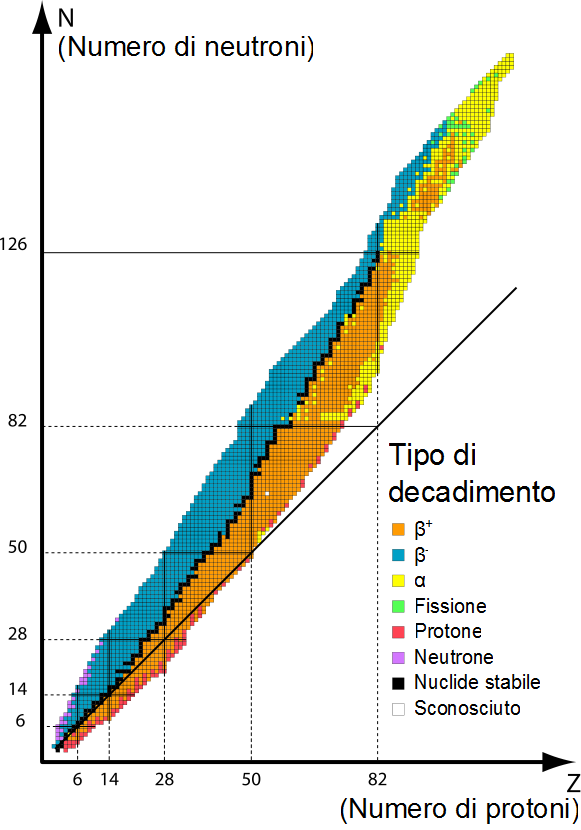
\includegraphics[width=7cm, keepaspectratio]{curvadistabilita.png}
		\caption{Curva di stabilità dei nuclei in funzione del numero di protoni e numero di neutroni. Sono rappresentati anche i decadimenti che tende a fare ogni elemento fuori dalla curva di stabilità.}
         \label{curvadistabilita}
\end{figure}

Due atomi si dicono:

\begin{itemize}
\item Isotopi, se hanno stesso numero atomico;
\item Isotoni, se hanno stesso numero di neutroni;
\item Isobari, se hanno stesso numero di massa.
\end{itemize}

Neutroni e protoni sono fermioni di spin $1/2$. Essi dunque si organizzano nel nucleo su livelli energetici in cui si dispongono a spin opposti.
Quando il numero di neutroni e protoni è pari, ogni livello energetico è riempito. Quando invece il loro numero è dispari, sono più probabili reazioni nucleari al fine di arrivare in livelli energetici più stabili. Ad esempio riempiendo i livelli energetici del $^{12}_5B$ ho un neutrone extra su un livello energetico più alto di quelli riempiti dai protoni. Questo elemento infatti decade $\beta$ nel $^{12}_6C$.
Per differenziare isotopi diversi si usano spettrometri di massa, in cui, sfruttando la forza di Lorenz generata da un campo magnetico, osservo la correlazione tra raggio di curvatura e massa dell'isotopo considerato.
Per misurare invece il raggio nucleare si osserva il pattern di diffrazione dello scattering di elettroni su tale nucleo. Graficando l'intensità dello scattering in funzione dell'angolo, ho la seguente relazione per il primo punto di minimo dell'andamento:

\begin{equation}
\sin \theta^*=0,16\frac{hc}{pcR}
\end{equation}

\begin{figure} []
\centering
		%% 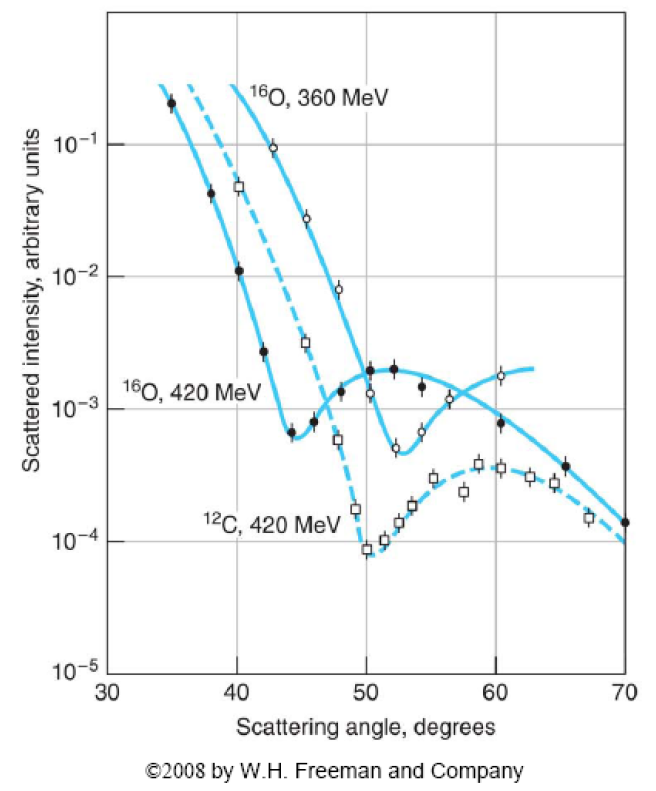
\includegraphics[width=7cm, keepaspectratio]{scatteringatomicradius.png}
		\caption{Andamento dell'angolo di scattering di elettroni su nuclei di ossigeno e carbonio.}
         \label{scatteringatomicradius}
\end{figure}

Da cui si può ricavare il raggio.

Empiricamente abbiamo la seguente legge che lega raggio nucleare e massa atomica:

\begin{equation}
R=1,15A^{1/3} (fm)
\end{equation}

Guardando la tavola periodica in Figura (\ref{atomicradii}) si può dire che gli elementi presenti in natura più grandi sono quelli in basso a sinistra più i gas nobili.
Consideriamo ora la densità nucleare. 

\begin{figure} []
\centering
		%% 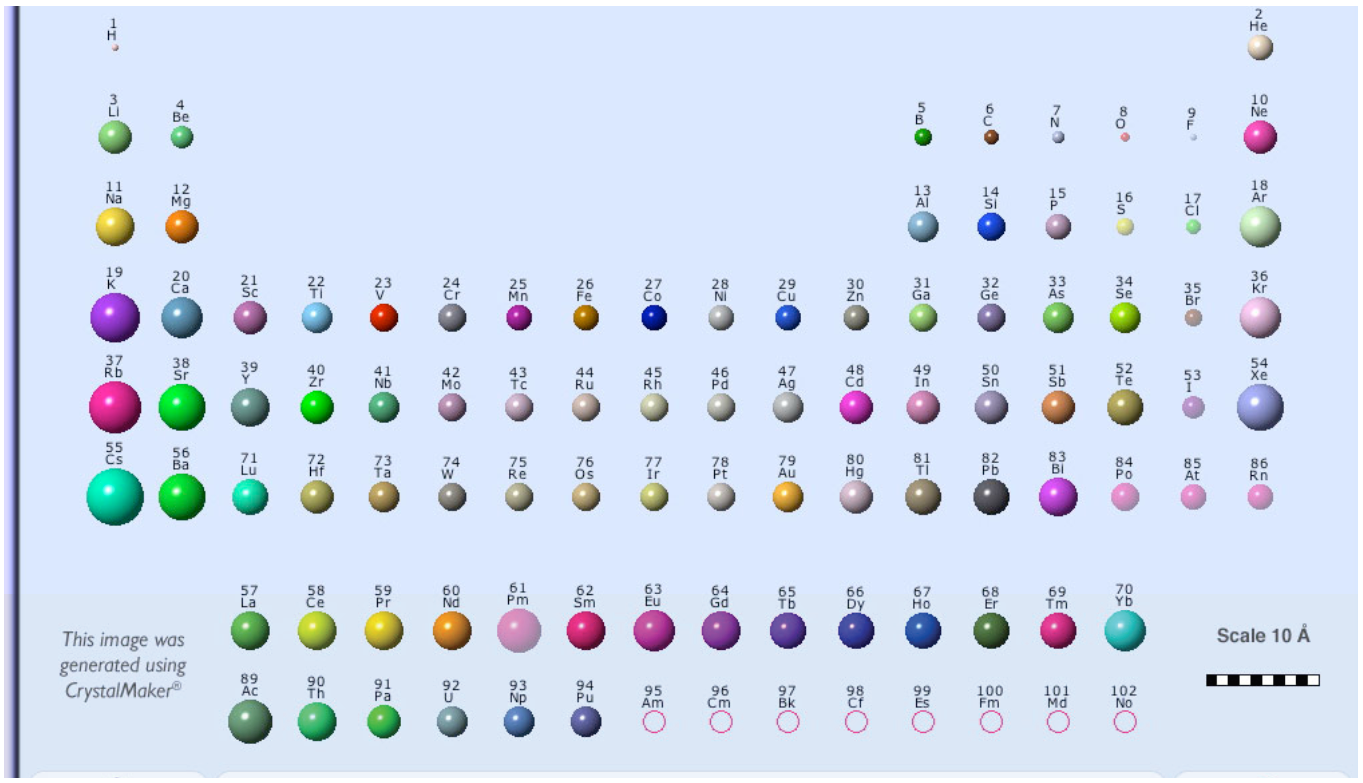
\includegraphics[width=16cm, keepaspectratio]{atomicradii.png}
		\caption{Tavola periodica. Sono evidenziati i raggi di ogni elemento.}
         \label{atomicradii}
\end{figure}

\begin{equation}
\rho=\frac{m}{\frac{4}{3}\pi R^3}=\frac{Am_p}{\frac{4}{3}\pi (1,15 A^{1/3})^3}=\frac{m_p}{\frac{4}{3}\pi 1,15^3 (fm^3)} = 10^{17} kg/m^3
\end{equation}

Ovvero essa è in prima approssimazione indipendente dal tipo di atomo. 
Altra verifica che questa sia la densità del nucleo atomico è che essa risulta essere la densità delle nane bianche, stelle in cui i nucleoni sono compressi uno contro l'altro.
                                                                                                                    
Per ricavare con maggiore precisione la massa atomica smettiamo di trascurare la differenza in massa tra neutroni e protoni e consideriamo anche l'energia di legame tra i nucleoni nel nucleo. Abbiamo allora che:

\begin{equation}
M(Z,A)=Z\times m_p+(A-Z)\times m_n-A\times BindingEnergy
\end{equation}

\textbf{Quarta Esperienza}

\begin{itemize}
\item \emph{Graficare la massa nucleare in funzione di Z per $A=18$ e $A=208$. Comparare il risultato con il grafico dei tempi di decadimento.}
\item \emph{Graficare Sp(Z) e Sn(Z) per $N=9$.}
\item \emph{Graficare Sp(N) e Sn(N) per $Z=33$.}
\end{itemize}


\section{Grandezze Importanti}

Quando un nucleo è instabile ha una certa probabilità per unità di tempo di decadere in un nucleo stabile, detta \emph{costante radioattiva} $\lambda$. 
Indicando con $N$ il numero di nuclei instabili, il numero medio di nuclei che decadono nell'unità di tempo è dato da $\lambda N$. Questa grandezza complessiva è detta \emph{attività}. Nel tempo tra $t$ e $t+dt$ il numero di nuclei varia al seguente modo:

\begin{equation}
\mathrm{d}N=-\lambda N \mathrm{d}t
\end{equation}

Risolvendo l'equazione differenziale si ottiene

\begin{equation}
N(t)=N(0)e^{-\lambda t}
\end{equation}

Osserviamo che il cosiddetto tempo di dimezzamento, ovvero il tempo al quale il numero di nuclei attivi è dimezzato, è dato da

\begin{equation}
\tau_{\frac{1}{2}}=\frac{\ln2}{\lambda}
\end{equation}

Ricordando che l'attività è definita come $\lambda N$, moltiplicando l'equazione precedente per $\lambda$ ottengo l'andamento temporale dell'attività:

\begin{equation}
A(t)=\lambda N(t)=A(0)e^{-\lambda t}
\end{equation}

L'unità di misura dell'attività era stata per convenzione stabilita essere il Curie, corrispondente a 37 miliardi di disintegrazioni al secondo, indicata con $\text{Ci}$. Essa è approssimativamente l'attività di un grammo di $^{226}\text{Ra}$.
Attualmente l'unità di misura più usata è diventata una disintegrazione al secondo, detta Bequerel, indicata $\text{Bq}$.
In laboratorio si usano di solito sorgenti dell'ordine del $\text{kBq}$. Dalle definizioni delle unità di misura segue il cambio:

\begin{equation}
1 \text{Ci} = 3,7 \times 10^{10} \text{Bq}
\end{equation}

Un atomo può decadere in canali diversi, ognuno con la sua vita media (e dunque la sua costante radioattiva). Allora si definisce la costante radioattiva totale $\lambda_{tot}=\sum \lambda_{i}$. Si introduce la branching fraction come $\text{BR}=\frac{\lambda_i}{\lambda_{tot}}$.\\

\emph{Nota: l'attività non tiene conto del tipo di fenomeno che sta avvenendo e di quante particelle genera. è un conto di quanti decadimenti avvengono, qualsiasi essi siano e qualunque numero di particelle producano. Per contare nello specifico il numero di un certo tipo di decadimento che avviene si usano gli Hz o i CPS (Counts Per Second)}\\

Si definiscono le seguenti grandezze importanti:
\begin{itemize}
\item Attività Specifica: $A_{sp}=\frac{\mathrm{d}A}{\mathrm{d}V}$
\item Standard Uptake Value (SUV): $\text{SUV}=\frac{A_{sp}(\text{tumore})}{A(\text{somministrata})}$ per renderla adimensionale si fa $\text{SUV}=\frac{A_{sp}(\text{tumore})}{A(\text{somministrata})\times \rho}m_{\text{paziente}}$
\item Tumor Non-tumor Ratio (TNR): $\text{TNR}=\frac{\text{SUV}(\text{tumore})}{\text{SUV}(\text{limitrofo})}$
\end{itemize}

In genere si cerca $\text{SUV}\sim5$

\section{Decadimenti $\alpha$}

Si definiscono decadimenti $\alpha$ quelli della seguente forma:

\begin{equation}
^A_Z X \longrightarrow ^{A-4}_{Z-2}Y + ^4_2He
\end{equation}

Siccome i prodotti di reazione sono due, nel sistema di riferimento dell'atomo che decade essi sono prodotti back to back con stesso impulso per conservazione della quantità di moto. Allora valgono le seguenti uguaglianze:

\begin{equation}
Q=T_y+T_{\alpha}=\frac{p^2}{2m_y}+\frac{p^2}{2m_{\alpha}}=\frac{m_{\alpha}}{m_y}T_{\alpha}+T_{\alpha}
\end{equation}

Da cui

\begin{equation}
T_{\alpha}=\frac{Q}{1+\frac{m_{\alpha}}{m_y}} 
\end{equation}

Da cui si deduce che per decadimenti di atomi molto massivi, in cui anche $Y$ è molto massivo, ho $T_{\alpha}\simeq Q$.\\

\emph{Nota: un decadimento può portare alla creazione di un prodotto che non è nel suo stato di spin nucleare fondamentale, ma ci decade emettendo raggi $\gamma$ }\\

Si osserva che c'è una relazione tra la vita media di un certo radionuclide e l'energia con cui vengono emesse le particelle $\alpha$: è la legge di Geiger-Nuttall:

\begin{equation}
\log \tau = a + b \log (E)
\end{equation}

\emph{Nota: si usa il $^{223}Ra$ per curare le metastasi nelle ossa o nella prostata perché mima il Calcio}

\section{Fissione Spontanea}

La fissione spontanea consiste nel decadimento di un nucleo pesante in due nuclei più leggeri con probabile produzione di neutroni. Esso è un processo altamente improbabile perché la barriera di potenziale da superare per farla avvenire è altissima. Il nucleo più leggero per cui si osserva è $^{226}Ra$, mentre quelli per cui la probabilità di fissione è paragonabile a quella di decadimento $\alpha$ sono alcuni isotopi dell'uranio. La fissione spontanea diventa dominante tra i branching ratio solo per $A>260$.
I prodotti di fissione sono normalmente lontani dalla curva di stabilità e decadono $\beta-$. 
Essi inoltre sono tra loro molto probabilmente asimmetrici: il valore più probabile di differenza di numero di massa tra i prodotti di fissione è circa $45$.

\begin{figure} []
\centering
		%% 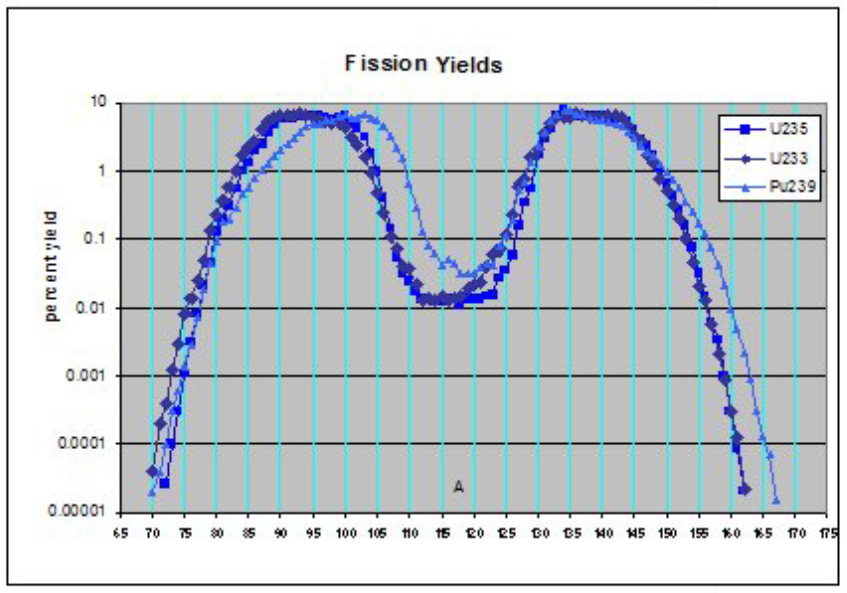
\includegraphics[width=12cm, keepaspectratio]{fissionyealds.png}
		\caption{Distribuzione di probabilità dei prodotti della fissione dell'$^{235}\text{U}$, del $^{233}\text{U}$ e del $^{239}\text{Pu}$. Si osserva che la produzione di due nuclei con massa simile è improbabile. Molto più probabile è la produzione di un nucleo pesante ed un nucleo leggero.}
         \label{fissionyealds}
\end{figure}

\section{Decadimenti Beta}

I decadimenti beta sono trasformazioni isobariche che avvengono per interazione debole e includono la presenza di un elettrone o un positrone. Sono di tre tipi:

\begin{equation}
\beta-: \qquad n \longrightarrow p + e^-+\bar{\nu_e}  \quad ovvero, atomicamente \quad  ^A_ZX \longrightarrow _{Z+1}^AY+e^-+\bar{\nu_e}
\end{equation}


\begin{equation}
\beta+: \qquad p \longrightarrow n + e^++\nu_e \quad ovvero, atomicamente \quad  ^A_ZX \longrightarrow _{Z-1}^AY+e^++\nu_e
\end{equation}


\begin{equation}
CE: \qquad p + e^- \longrightarrow n + \nu_e \quad ovvero, atomicamente \quad  ^A_ZX+e^- \longrightarrow _{Z-1}^AY+\nu_e
\end{equation}

Osserviamo che tutte sono reazioni che conservano il numero di massa totale dell'atomo ma cambiano il suo numero atomico.
Fuori dal nucleo è impossibile che avvengano decadimenti $\beta+$ perché la massa del protone è inferiore a quella del neutrone. Invece le reazioni $\beta-$ avvengono velocissime fuori dal nucleo, ed è per questo che non esistono neutroni liberi.
Osserviamo inoltre che quando avviene cattura elettronica tutti gli altri elettroni devono riaggiustarsi scendendo ai livelli inferiori, emettendo intensa radiazione X.
Per i decadimenti $\alpha$ avevamo visto che siccome c'era un prodotto massivo e l'$\alpha$ leggera allora il Q value andava tutto all'energia cinetica della particella $\alpha$. In questo caso invece sono due i prodotti leggeri: neutrino ed elettrone o positrone.

 Come si può vedere nelle figure (\ref{qbetapiu}) e (\ref{qbetameno}) le distribuzioni di energia con cui vengono prodotti elettroni e positroni sono diverse perché è diverso il loro Q value. Nelle seguenti equazioni le maiuscole sono le masse atomiche, minuscole le masse nucleari (la differenza è la massa degli elettroni).

\begin{figure} []
\centering
		%% 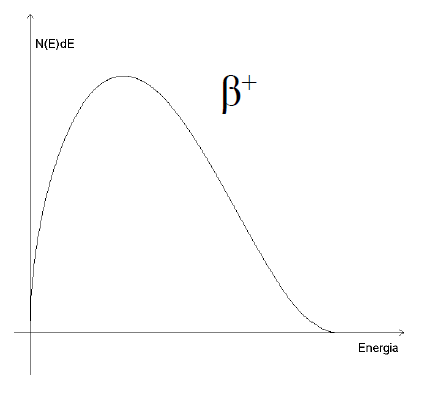
\includegraphics[width=5cm, keepaspectratio]{qbetapiu.png}
		\caption{Distribuzione dell'energia del positrone prodotto in un decadimento $\beta+$. La probabilità che esso abbia energia nulla è zero, perché}
         \label{qbetapiu}
\end{figure}

\begin{figure} []
\centering
		%% 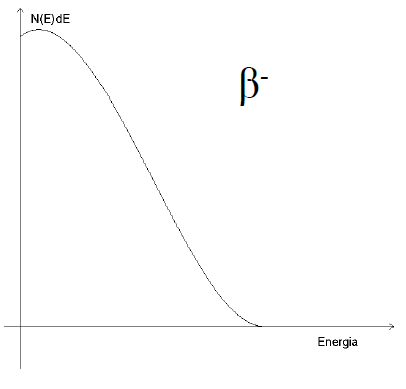
\includegraphics[width=5cm, keepaspectratio]{qbetameno.png}
		\caption{Distribuzione dell'energia dell'elettrone prodotto in un decadimento $\beta-$.}
         \label{qbetameno}
\end{figure}

\begin{equation}
M_x=m_x+Zm_e 	\qquad M_y=m_y+(Z+1)m_e
\end{equation}

\begin{equation}
Q_{\beta^-}=m_x-m_y-m_e
\end{equation}

è facile osservare che $M_x-M_y=m_x-m_y-m_e$. Allora possiamo dire:

\begin{equation}
Q_{\beta^-}=M_x-M_y
\end{equation}

Ciò ci dice anche che condizione necessaria e sufficiente a far avvenire un decadimento $\beta^-$ è che la massa del nucleo padre sia maggiore della massa del nucleo figlio.

Per il decadimento $\beta^+$ invece:

\begin{equation}
M_x=m_x+Zm_e \qquad M_y=m_y+(Z-1)m_e
\end{equation}

\begin{equation}
Q_{\beta^+}=m_x-m_y-m_e
\end{equation}

Si osserva facilmente che $M_x-M_y=m_x-m_y+m_e=Q_{\beta^+}+2m_e$.
Ovvero

\begin{equation}
Q_{\beta^+}=M_x-M_y-2m_e
\end{equation}

Allora condizione necessaria e sufficiente a far avvenire un decadimento $\beta^+$ è che la differenza di masse atomiche tra nucleo padre e nucleo figlio sia almeno due volte la massa dell'elettrone: $M_x-M_y>2m_e$.

In natura, con l'eccezione del $^{40}K$, non esistono radionuclidi che decadono $\beta^+$, vengono prodotti artificialmente.

Il punto estremo della distribuzione di energie degli elettroni in queste due reazioni è detto End Point, ed è dato da quegli elettroni che estraggono tutta l'energia dal Q value.

Un nucleo può \emph{catturare un elettrone} dalla shell atomica, trasformare un protone in neutrone ed emettere un neutrino con la seguente reazione:

\begin{equation}
^A_ZX+e^- \longrightarrow _{Z-1}^AY+\nu_e
\end{equation}

Data la pesantezza di $Y$ rispetto al neutrino, quest'ultimo viene praticamente emesso sempre con la stessa energia. In questo caso il Q value ci pone il seguente vincolo:

\begin{equation}
M_x+m_e>M_y
\end{equation}

Allora riassumendo in scala di energie crescente i decadimenti possibili sono i seguenti:

\begin{itemize}
\item Cattura Elettronica se $M_x-M_y>-m_e$
\item Decadimento $\beta^-$ se $M_x-M_y>0$
\item Decadimento $\beta^+$ se $M_x-M_y>2m_e$
\item Decadimento $\alpha$ se $M_x-M_y>m_{\alpha}$
\end{itemize}

\textbf{Quinta Esperienza}\\

\begin{itemize}
\item \emph{Trovare una lista di isotopi di C, Na, F, P, Ga, I, Re, Lu, Y e Sr con decadimenti $\beta+$ e $\beta-$ dominanti con un tempo di dimezzamento compreso tra 1 minuto e 10 giorni.}
\item \emph{Per ogni isotopo scrivere tempo di dimezzamento, end point e range proiettato per energie che siano pari a metà dell'end-point.}
\end{itemize}



Un applicazione del decadimento $\beta^-$ è la Brachioterapia \cite{Brachioterapia}, che consiste nello spalmare pomate emettenti elettroni sui tumori. Il LET degli elettroni abbiamo visto che è molto corto e concentrato all'inizio grazie al multiple scattering. Si cercano elementi ad alto End Point. Gli elementi più usati sono:
\begin{itemize}
\item $^{90}\text{Y}$ per il fegato,
\item $^{188}\text{Re}$ per la pelle,
\item $^{32}\text{P}$ per il cervello,
\item $^{90}\text{Sr}$ per fegato e polmoni.
\end{itemize}

Ognuno di questi ha endpoint dell'ordine del MeV e range proiettato dell'ordine del millimetro.
Si usa inoltre per la terapia radiometabolica, in cui i radionuclidi sono attaccati a molecole che vengono metabolizzate dai tumori. Gli elementi più usati sono:

\begin{itemize}
\item $^{90}\text{Y}$ per i tumori neuroendocrini,
\item $^{131}\text{I}$ $^{132}\text{I}$ per la tiroide,
\item $^{177}\text{Lu}$ per i tumori neuroendocrini.
\end{itemize}

La tipica iniezione è di $3 \text{MBq/kg}$

Altra applicazione è la \emph{Chirurgia Radioguidata} in cui si inserisce un tracciatore che decade $\beta^-$, tipo $^{90}\text{Y}$, e un detector di elettroni da passare sul punto da operare. Lo svantaggio è che bisogna sviluppare un tracciatore specifico per ogni caso. Quì è stato inventato PROBE.

Ancora un'altra applicazione: la PET usa decadimenti $\beta^+$ insieme a radiofarmaci funzionali per fare uno scan delle coppie gamma prodotte dal positronio. In questo caso voglio basso End Point. Gli elementi più usati sono:

\begin{itemize}
\item $^{18}\text{F}$ generico,
\item $^{11}\text{C}$ per prostata e cervello,
\item $^{68}\text{Ga}$ per tumori neuroendocrini,
\item $^{13}\text{N}$ per la pelle.
\end{itemize}

Infine osservando i prodotti di reazione posso fare una valutazione della Dose che ha attraversato il paziente.

\section{Emissione $\gamma$}

I nuclei risultanti da decadimenti $\beta$ possono trovarsi in stati diversi da quello fondamentale. In tal caso esso cadrà negli stati più bassi in energia emettendo raggi $\gamma$. La transizione può avvenire con un unico salto e produzione di un fotone molto energetico, o con più salti intermedi e la produzione di una cascata di raggi $\gamma$. Si dice emissione gamma e non decadimento gamma perché non c'è correlazione tra il numero di atomi che scende allo stato fondamentale e il numero di fotoni emessi. La vita media di tali stati è dell'ordine del picosecondo, poco più di quella dei decadimenti beta. Ci sono alcune eccezioni, date da stati metastabili, tipo il $^{99m}\text{Tc}$ metastabile prodotto dal decadimento beta- del $^{99}\text{Mo}$ per cui la vita media è 6 ore.
L'emissione gamma è in competizione con un altro fenomeno che può avvenire con un nucleo in stato eccitato: la \emph{Conversione Interna}. Ciò consiste nel fenomeno per cui l'energia in eccesso del nucleo viene direttamente trasferita ad un elettrone che viene ionizzato ed assume energia finale:

\begin{equation}
E_{e^-}=E_{s.eccitato}-I
\end{equation}

\emph{Nota: Per possibili decadimenti gamma con le loro probabilità si consulta questo sito: \\http://nucleardata.nuclear.lu.se/toi/nucSearch.asp }\\

Un'applicazione di questo fenomeno è la SPECT (Single Photon Emission Computed Tomography). Ogni decadimento porta all'emissione di un fotone. Si mette in circolazione una sostanza radioattiva che va nell'organo di interesse ed emette un fotone. Il rilevatore mi dice energia e direzione del fotone usando varie fessure che selezionano la direzione. Voglio un cammino libero di 10cm così che riesca ad uscire dal corpo del paziente. Il rilevatore deve essere un calorimetro molto assorbente e con setti molto lunghi e densi. L'elemento che cerco è il $^{99m}\text{Tc}$.

Altra applicazione è la Teragnostica: si fa con elementi che decadono sia $\beta-$ che $\gamma$ così da fare terapia e diagnostica rispettivamente. Elementi utili a ciò sono $^{177}\text{Lu}$ e $^{131}\text{I}$.

Ai fini di monitorare la dose come visto prima si possono usare gli elettroni dei decadimenti beta ma ci mettono troppo ad uscire. Invece i raggi $\gamma$ prodotti nella reazione danno informazioni immediate su dove si sta rilasciando la dose.

Ultima applicazione è la radioterapia con il cobalto. Il $^{60}\text{Co}$ decade $\beta-$ e i suoi prodotti decadono $\gamma$. Allora il paziente riceve un elettrone e due fotoni. I pazienti inoltre vedono live la loro risonanza magnetica e possono aggiustarsi per rimanere nella zona di interesse. La dose è monitorata live quindi se il paziente si muove e fa uscire il target dalla zona di interesse il fascio si spegne.

\section{Equilibrio Secolare}

Un fenomeno interessante si verifica quando un nucleo padre con tempo di vita medio $\tau_f$ decade in un nucleo figlia con tempo di vita $\tau_d$ una frazione $\Phi$ di volte. Ricordando che abbiamo definito l'attività come $A=\lambda N=\frac{N(0)}{\tau}e^{-t/\tau}$, segue che, guardando il numero totale di nuclei figlie che ho, esso aumenta per produzione dal padre e diminuisce per decadimento:

\begin{equation}
\frac{dN_d}{dt}=-\Phi \frac{dN_f}{dt} - \frac{\partial N_d}{\partial t} = \Phi \frac{N_f}{\tau_f} - \frac{N_d}{\tau_d}
\end{equation}

Integrando ottengo

\begin{equation}
N_d(t)=\frac{\Phi}{\frac{\tau_f}{\tau_d}-1}N_f(0)(e^{-t/\tau_f}-e^{-t/\tau_d})
\end{equation}

Per finire rendiamola un'attività dividendo per $\tau_d$, ma esprimiamo $A_f(0)$ al posto di $N_f(0)$. Otteniamo:

\begin{equation}
A_d(t)=\frac{\Phi}{\frac{\tau_f}{\tau_d}-1}A_f(0)\frac{\tau_f}{\tau_d}(e^{-t/\tau_f}-e^{-t/\tau_d}) =\frac{\Phi}{1-\frac{\tau_d}{\tau_f}}A_f(0)(e^{-t/\tau_f}-e^{-t/\tau_d})
\end{equation}

Analizziamo adesso i casi limite. Se $\tau_d << t << \tau_f$, come nel $^{99}\text{Mo} \rightarrow ^{99m}\text{Tc}$, avrò:

\begin{equation}
A_d(t)=\Phi A_f(t)
\end{equation}

Ovvero l'attività del nucleo figlia sarà solo scalata di un certo fattore rispetto a quella del padre.

Invece quando ho $\tau_f \sim t << \tau_d$ , come nel $^{223}\text{Ra}$, ottengo:

\begin{equation}
A_d(t)=\Phi \frac{\tau_f}{\tau_d}A_f(0)(\-e^{-t/\tau_f})
\end{equation}

Torniamo al primo caso e osserviamo cosa succede se estraiamo i nuclei figlie dopo una vita media $\tau_d$. Grafico.

Si possono creare dei generatori continui di Tecnezio con macchinari contenenti Molibdato $^{99}\text{MoO}_4^{2-}$ e Pertecnato $^{99m}\text{TcO}_4^-$.
Altri esempi sono le famiglie naturali dell'$^{238}\text{U}$, $^{232}\text{Th}$ e $^{235}\text{U}$.  Le attività di una famiglia sono tutte legate tra loro dalle equazioni differenziali di Bateman.

Osserviamo un esempio: $^{90}\text{Sr} \rightarrow ^{90}\text{Y} \rightarrow ^{90}\text{Zr}$. Quando prendo una certa quantità di Becquerel di $^{90}\text{Sr}$ sto prendendo anche la stessa attività di ittrio a meno di un fattore $\Phi$. Qui si vede la differenza tra rate e attività: prendendo $1 \ Bq$ di stronzio ho $2 \ kHz$ di produzione di elettroni, uno dal decadimento dello Stronzio e uno dal decadimento dell'Ittrio. \\

\textbf{Sesta Esperienza}\\

\emph{Trovare coppie di nuclei padre-figlia in cui:}
\begin{itemize}
\item \emph{La figlia decade $\beta$ con $\tau\sim1-100\text{hr}$}
\item \emph{Il padre decade con $\tau\sim100\text{d}-10\text{y}$}
\end{itemize}

